\chapter{PERANCANGAN PERANGKAT LUNAK}
\label{chap:perancangan perangkat lunak}

Pada bab ini akan dibahas tentang penjelasan perancangan perangkat lunak untuk membuat \textit{Twitter Bot} untuk mencari jalur transportasi publik sesuai analisa yang sudah dibahas pada bab 3.

\section{Perancangan Perangkat Lunak}

\subsection{Perancangan Kelas}
Pada subbab ini akan dibahas rancangan kelas dan \textit{method} yang akan dibuat pada aplikasi Pembuatan Twitter Bot untuk Mencari Jalur Transportasi Publik. Untuk lebih jelas mengenai kelas yang ada pada aplikasi ini, penulis menyajikan gambar diagram kelas yang dapat dilihat pada gambar ...

\begin{figure}[htbp]
	\centering
		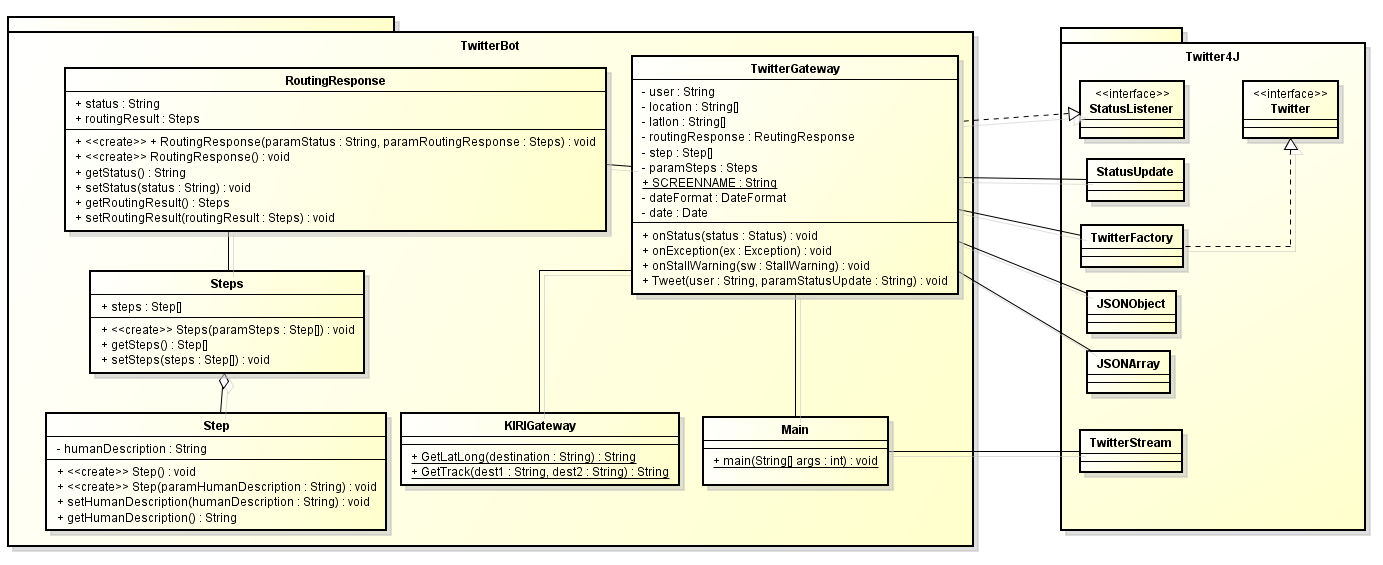
\includegraphics[width=1.00\textwidth]{C:/Skripsi/doc/DokumenSkripsi/Gambar/classDiagramSkripsi.PNG}
	\caption{Class Diagram Pembuatan Twitter Bot untuk Mencari Jalur Transportasi Publik}
	\label{fig:classDiagramSkripsi}
\end{figure}


\begin{itemize}
		\item Kelas Main, merupakan kelas yang berfungsi untuk membuat koneksi dengan Twitter ketika program dijalankan.
		
				\begin{itemize}
							\item Method
							
									\begin{itemize}
												\item public static void main(String[] args), merupakan method main untuk menjalankan program.
										
									\end{itemize}
				\end{itemize}
		
		\item Kelas Twitter Gateway, merupakan kelas yang berfungsi untuk menangkap dan membalas Tweet
		
		
				\begin{itemize}
							\item Atribut
							
							
									\begin{itemize}
												\item String user, digunakan untuk menampung nama user
												\item String location[], berupa array yang digunakan untuk menampung lokasi awal dan lokasi tujuan
												\item String latlon[], berupa array yang digunakan untuk menampung koordinat lokasi awal dan koordinat lokasi tujuan
												\item RoutingResponse routingResponse, merupakan variable yang digunakan untuk menampung hasil yang diberikan oleh KIRI API
												\item Step[] step, berupa array yang berguna untung menampung informasi dari langkah-langkah informasi perjalanan
												\item Steps paramSteps, marupakan variable yang berguna untung menampung semua step.
									\end{itemize}
							
							\item Method
							
									\begin{itemize}
												\item public void onStatus(Status status), merupakan method yang menangkap tweet dan memproses tweet tersebut
												\item public void onDeletionNotice(StatusDeletionNotice statusDeletionNotice),
												\item public void onTrackLimitationNotice(int numberOfLimitedStatuses)
												\item public void onScrubGeo(long userId, long upToStatusId)
												\item public void onException(Exception ex), merupakan method yang berguna untuk menangkap \textit{exception}
												\item public void onStallWarning(StallWarning sw)
												\item public void Tweet(String user, String paramStatusUpdate), merupakan method untuk melakukan tweet balasan kepada user yang dituju.
									\end{itemize}
				\end{itemize}
		
		\item Kelas KIRIGateway, merupakan kelas untuk memanggil KIRI API
		
		
				\begin{itemize}
							\item Method
							
							
									\begin{itemize}
												\item public static String GetLatLong(String destination), method yang digunakan untuk mencari koordinat dari suatu lokasi
												\item public static String GetTrack(String dest1, String dest2), method yang digunakan untuk memcari jalur transportasi publik dari lokasi awal ke lokasi tujuan
									\end{itemize}
				\end{itemize}
		
		
		\item Kelas RoutingResult, merupakan kelas untuk menampung hasil kembalian dari KIRI API
		
		
				\begin{itemize}
							\item Atribute
					
					
									\begin{itemize}
												\item status, digunakan untuk menyimpan apakah status ok atau tidak
												\item routingResult, digunakan untuk menyimpan langkah-langkah perjalanan
									\end{itemize}
					
							\item Method
					
					
									\begin{itemize}
												\item public RoutingResponse(String paramStatus, Steps paramRoutingResult), merupakan konstruktor dari kelas RoutingResult yang memiliki parameter untuk status dan routingResult.
												\item public RoutingResponse(), merupakan konstruktor dari kelas RoutingResult.
												\item public String getStatus(), merupakan \textit{getter} dari atribut status.
												\item public void setStatus(String status), merupakan \textit{setter} dari atribut status.
												\item public Steps getRoutingResult(), merupakan \textit{getter} dari atribut routingResult.
												\item public void setRoutingResult(Steps routingResult), merupakan \textit{setter} dari atribut routingResult.
									\end{itemize}
				\end{itemize}
		
		\item Kelas Steps, merupakan kelas untuk menampung kumpulan step. (Merupakan pecahan dari hasil RoutingResult)
		
		
				\begin{itemize}
							\item Atribute
					
					
									\begin{itemize}
												\item Step[] steps, merupakan atribut yang berisi \textit{array} dari step
									\end{itemize}
					
							\item Method
					
					
									\begin{itemize}
												\item public Steps(Step[] paramSteps), merupakan konstruktor dari kelas Steps.
												\item public Step[] getSteps(), merupakan \textit{getter} dari atribut steps.
												\item public void setSteps(Step[] steps), merupakan \textit{setter} dari atribut steps.
									\end{itemize}
				\end{itemize}
		
		\item Kelas Step, merupakan kelas untuk menampung jalur perjalanan / menampung hasil dari KIRI API
		
		
				\begin{itemize}
							\item Atribute
					
					
									\begin{itemize}
												\item String humanDescription, merupakan atribut untuk menjelaskan cara perjalanan yang bahasanya dimengerti oleh pengguna.
									\end{itemize}
					
							\item Method
					
					
									\begin{itemize}
												\item public Step(), merupakan konstruktor dari kelas Step.
												\item public Step(String paramHumanDescription), merupakan konstruktor dari kelas Step yang memiliki parameter humanDescription.
												\item public String getHumanDescription(), merupakan \textit{getter} dari atribut humanDescription.
												\item public void setHumanDescription(String humanDescription), merupakan \textit{setter} dari atribut humanDescription.
									\end{itemize}
				\end{itemize}
\end{itemize}




\subsection{Sequence Diagram}

Pada subbab ini, akan dijelaskan alur program dengan menggunakan \textit{sequence diagram} pada ...

\begin{figure}[htbp]
	\centering
		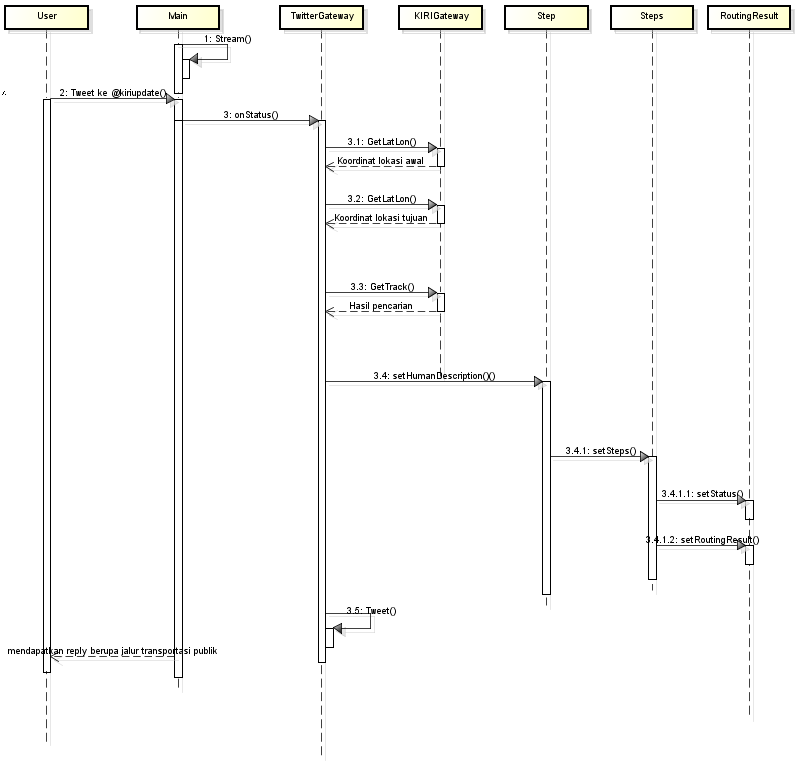
\includegraphics[width=1.00\textwidth]{C:/Skripsi/doc/DokumenSkripsi/Gambar/diagramSequence2.PNG}
	\caption{Sequence Diagram Pembuatan Twitter Bot untuk Mencari Jalur Transportasi Publik}
	\label{fig:diagramSequence2}
\end{figure}


Pertama, program akan menjalankan melakukan \textit{streaming} pada saat kelas \textit{main} dijalankan. Kelas \textit{main} akan membuka gerbang untuk mengakses \textit{Twitter API}, lalu \textit{steaming} akan dilakukan dengan melakukan \textit{track} dengan katakunci @kiriupdate. Program akan terus menangkap semua \textit{tweet} yang dirujuk kepada @kiriupdate.

Kelas TwitterGateway akan memproses \textit{tweet} ketika terdapat \textit{tweet} yang dirujuk (\textit{mention}) kepada @kiriupdate. Melalui \textit{method onStatus} maka \textit{tweet} tersebut akan disimpan nama user pengirimnya, dan diperiksa apakah \textit{tweet} tersebut dilakukan untuk mencari jalur transportasi publik atau bukan. Jika benar maka alamat dari lokasi awal dan lokasi tujuan akan disimpan lalu akan dicari koordinat dari masing-masing lokasi menggunakan KIRI API. Proses pencarian koordinat ini dilakukan oleh kelas KIRIGateway.

Kelas KIRIGateway akan memanggil \textit{method GetLatLon} untuk pencarian koordinat. Setelah didapatkan koordinat dari masing-masing lokasi maka kelas TwitterGateway akan mengolahnya terlebih dahulu karena kembalian dari \textit{method GetLatLon} ini berupa JSON. Setelah itu maka hasilnya akan dikembalikan kepada kelas KIRIGateway untuk dicari jalurnya menggunakan \textit{method GetTrack}. Hasil dari \textit{method GetTrack} lalu disimpan pada atribut \textit{step, steps}, dan \textit{routingResult}.

Setelah semuanya selesai maka langkah-langkah jalur transportasi publik siap di \textit{reply}. Kelas TwitterGateway memanggil \textit{method Tweet} untuk di-\textit{reply tweet} yang berisikan langkah-langkah dari jalur transportasi publik. \textit{Tweet} akan di-\textit{reply} satu per satu sesuai dengan banyaknya \textit{step} yang ada. Setelah semuanya selesai, program akan menunggu \textit{tweet} selanjutnya.

\subsection{Perancangan Antar Muka}

Pada sub bab ini akan dibahas mengenai antarmuka pada aplikasi Pembuatan Twitter Bot untuk Mencari Jalur Transportasi Publik. Aplikasi ini memiliki perancangan antar muka berbasis \textit{text}. Sedangkan user dapat mencoba aplikasi ini secara langsung menggunakan Twitter, baik menggunakan website Twitter ataupun aplikasi Twitter.

